\باب{مقناطیسی دور}  
\حصہ{مزاحمت او ہچکچاہټ}
پہ شکل \حوالہ{شکل_مقناطیسی_دور_مزاحمت_ہچکچاہٹ} کښ ښودلے شوی موصل خختے  د اوږدوالی پہ سمت مزاحمت 
\begin{align}\label{مساوات_مقناطیسی_دور_مزاحمت_کی_تعریف}
R=\frac{l }{\sigma A}
\end{align}
دے چہ \عددیء{\sigma} پکښ د خختے موصلیت ښائی۔کہ ھم د دغہ خختے مقناطیسی مستقل الف وی نو د خختے ہچکچاہټ  د اوږدوالی پہ سمت کښ بہ 
\begin{figure}
\centering
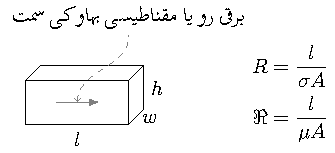
\includegraphics{figMagneticCircuitsResistanceAndReluctance}
\caption{مزاحمت اور ہچکچاہٹ}
\label{شکل_مقناطیسی_دور_مزاحمت_ہچکچاہٹ}
\end{figure}
وی۔مقناطیسی مستقل عموماً د خالی خلاء د مقناطیسی مستقل پہ نسبت لیکلے شی یعنی 

چہ پکښ الف تہ جزو مقناطیسی مستقل وئیلے شی۔د ہچکچاہټ اکائی ایمپیئر-چکر فی ویبر دہ۔د دے اکائی وضاحت بہ مخکښ راشی۔ 

\ابتدا{مثال}
پہ شکل کښ د خختے ہچکچاہټ حاصل کړے۔
\انتہا{مثال}


\حصہ{کثافت برقی رو او د برقی میدان شدت}
شکل الف کښ د سلاخ د دوو سرو تر ځامینځ الف برقی دباو ورکړے شوے دے۔د اوہم قانون مطابق پہ سلاخ کښ د برقی رو مقدار بہ

وی۔د مساوات الف پہ مدد سرہ مونږ دا برقی رو داسے ہم لیکلے شو۔


دا داسے ہم لیکلے شی۔

دا د اوہم مساوات بل شکل دے چہ پکښ 


دی۔کہ پہ شکل کښ د الف طول ب وی، د ت طول ټ وی او د دے دواړو سمت الف وی نو بیا دا مساوات 

لیکلے شی۔

د شکل نہ ښکارہ دہ چہ برقی رو د سلاخ د رقبہ عمودی تراش نہ تیریږی۔دا شان مساوات الف کښ ب د برقی رو کثافت ظاہروی۔ہم پہ دے وجہ ب تہ کثافت برقی رو وئیلے شی۔ہم دغہ شان الف برقی دباو فی اکائی فاصلہ ظاہروی۔ہم پہ دے وجہ الف تہ د برقی میدان شدت وئیلے شی۔چہ کوم ځائے د متن نہ واضحہ وی نو ھعہ ځائے دا نوم وړوکے کړے شی او ورتہ میدانی شدت وئیلے شی۔ 

\حصہ{برقی دور}
د شکل-الف دپارہ مونګ لیکلے شو
\begin{align}
v&=\Delta v_w+ v_{RL}\\
i&=\frac{v-\Delta v_w}{R_L}
\intertext{\RL{چہ پکښ}}
\Delta v_w&=i R_w 
\end{align}
دہ۔د تانبے موصلیت الف دے چہ ب پکښ د موصلیت اکائی دہ۔دا شان د تانبے نہ د جوړ تار د مزاحمت قیمت د نظرانداز کولو قابل وی۔پہ دے وجہ مونږ \عددیء{\Delta v_w \to 0} لیکلے شو۔د دے مطلب دے


